%%%%%%%%%%%%%%%%%%%%%%%%
%
% $Autor: Srikanth Nanda $
% $Datum: 2024-12-05 $
% $Pfad: ML24-06-Magic-Wand-with-an-Arduino-Nano-33-BLE-Sense/report/Contents/en/Application.tex $
% $Version:### $
%
%%%%%%%%%%%%%%%%%%%%%%%%

\chapter{Application}

\section{Application of Magic Wand with an Arduino Nano 33 BLE Sense}
\label{Application}
The Magic Wand project aims to develop a handheld device that can interact with a computer or other systems through Bluetooth Low Energy (BLE) technology. 
The device is designed to recognize specific gestures made by the user and translate them into commands or actions. 
The Magic Wand uses the Arduino Nano 33 BLE Sense board, which is equipped with various sensors, including an accelerometer, gyroscope, magnetometer, and temperature sensor. 
These sensors allow the device to capture the user's movements and orientation in real-time, enabling gesture recognition and interaction with the system. 
The Magic Wand project involves programming the Arduino Nano 33 BLE Sense board to read sensor data, process the data to recognize gestures, and communicate wirelessly with a computer or other devices. 
The project also includes developing a user interface or application on the computer to receive and interpret the gesture commands sent by the Magic Wand. 
The Magic Wand project demonstrates the capabilities of the Arduino Nano 33 BLE Sense board and explores the possibilities of gesture-based human-computer interaction using BLE technology. 
The project has various applications in fields such as gaming, virtual reality, human-computer interaction, and assistive technology. 
By developing a responsive and efficient gesture recognition system, the Magic Wand project aims to provide an intuitive and interactive way for users to control and interact with digital systems and devices. 
The project also highlights the potential of using low-cost and accessible hardware platforms like the Arduino Nano 33 BLE Sense for developing innovative and interactive applications in various domains. 
The Magic Wand project showcases the power of combining hardware, software, and sensor technologies to create novel and engaging user experiences and demonstrates the possibilities of using gesture-based interaction as a means of human-computer communication. 
The project also emphasizes the importance of user-centered design and usability testing to ensure that the Magic Wand is intuitive, easy to use, and accessible to a wide range of users. 
By exploring the capabilities of the Arduino Nano 33 BLE Sense board and developing a gesture recognition system, the Magic Wand project aims to inspire creativity, innovation, and exploration in the field of interactive technology and human-computer interaction. 
The Magic Wand project represents an exciting opportunity to experiment with sensor technologies, wireless communication, and gesture recognition algorithms and to create a unique and engaging user experience that combines physical movement with digital interaction. 
The project has the potential to open up new possibilities for interactive technology and to inspire future projects and applications that leverage the capabilities of the Arduino Nano 33 BLE Sense board and other sensor-based platforms. 
\section{Problem}
The project represents an exciting challenge in interactive technology
using board Arduino Nano 33 BLE Sense, whereby the project derived is
referred to as the Magic Wand. This project aims to develop and implement a handheld device similar to the magic wand by using the board
Arduino Nano 33 BLE Sense due to its characteristics such as wireless
communication implementation. The wand is expected to interact with
a suitable system, such as a computer, through the implementation of
Bluetooth Low Energy (BLE) technologies. The challenge would be to
develop a responsive and efficient gesture recognition system that can
remap the wand movement of the user into actual commands. 
Moreover, the project might incorporate sensors like accelerometers or gyroscopes for accurately capturing and interpreting gestures. 
Thus, Successful implementation requires an understanding of programming Arduino, sensor integration, and BLE communication protocols. 
In this Magic Wand project, it will be essential to resolve the intricacies by documenting
the board Arduino Nano 33 BLE Sense, sensor datasheets, and other
relevant online resources covering gesture recognition algorithms. For this
reason, the project not only comes up with a fantastic and exciting way
of testing board Arduino Nano 33 BLE Sense capabilities but also opens
new horizons in gesture-based human-computer interaction.

\section{Data Acquisition}
\subsection{Database}

	In the lack of pre-existing databases adapted to our specific model, we developed a new database for our Magic Wand project. The information is organised as a.txt file and contains raw data from accelerometer readings taken by the Arduino Nano 33 BLE Sense. Recognising the inherent heterogeneity in how people capture gestures, we asked three members of our group to contribute, resulting in a richer and more diverse dataset. Each participant scrupulously documented at least 50 trials of each gesture W, O, and L to ensure a complete representation of gesture variability. This strategy takes advantage of the distinct hand movements of three different users, improving the database's accuracy, efficiency, and efficacy. \cite{War:2020}
	
	In the next part of our project, named Data Preparation and Quality," we intend to process the raw data collected from the database. This includes identifying and resolving outliers as needed, as well as further refining the dataset to ensure optimal performance when training our machine learning model. The comprehensive quality of our dataset, enriched by diverse contributions and purposefully limited in size, provides a solid foundation for the project's succeeding phases, promising an effective and adaptable model for Magic Wand gesture identification. Detailed Information about database in teh section \ref{Database}.
	

\subsection{Data Preparation}

	This section discusses how to shape our data and how we can use it for training. Our data model will recognise three gestures: wing, slope and ring. Since we do not intend to use existing databases to prepare the data, we will give multiple inputs for a single gesture and save it as model data for the gesture. When a gesture, for example - ``wing'' is waved using the wand, the accelerometer present in the microcontroller detects the movement by using the coordinates in the x,y and z axes. The exact process is repeated multiple times for the dataset to be as large as possible. Creating a database with more inputs allows the data model to be more accurate and provides better and more efficient results. The exact process is repeated for the remaining gestures, namely ring, slope and unknown. 
	With the data available for the above gestures, we can use it to train a model. The available data is split into two sets, namely training data and test data.

	The major challenge while preparing data can be the presence of outliers or anomalies with unexpected values. This can be overcome by feeding our model with more data so that the model is efficient.\cite{War:2020}

	The different steps involved in preparing data can be as follows according to \cite{War:2020}

\begin{description}
	\item[Understanding the problem]  The problem, which in our case is the collection of data consisting of gestures. The main problem is divided into many parts for easy data preparation.
	\item[Preparation of data] The step deals with converting the raw data into machine learning language that the compiler can interpret.
	\item[Evaluation of data] This step deals with evaluating the model after the collection of the necessary data. This data is then checked for correctness, and analysis is done according to the accuracy of the output obtained. 
	\item[Finalizing the data] The model is tested with various parameters and the data is validated. If the results obtained are according to our requirements, the resulting dataset is finalized.
\end{description}

	The same steps are repeated for various gestures and the final database is created.

\subsubsection{Preparation of Datasets for the Magic Wand}

	Since the amount of data required for the creation of a database is very small, the database will be prepared by us. The first set of data that we are trying to capture the movement is for the gesture ``W''. The steps involved in capturing a W are mentioned below. \cite{War:2020}

\vspace{5mm}
\begin{center}
	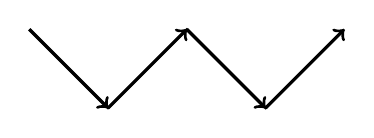
\begin{tikzpicture}
		% define point
		\coordinate (A)  at (1, 1);
		\coordinate (O)  at (2, 0);
		\coordinate (B)  at (3, 1);
		\coordinate (C)  at  (4,0);
		\coordinate (D) at  (5,1);
		% angle  
		\draw[thick] (A) -- (O) -- (B) -- (C)-- (D);
		%	\draw pic[draw=black,eccentricity=2.9]
		%\pic [draw,"$\alpha_1$",angle radius=20,->,angle eccentricity=1.4]
		%  {angle = B--O--A};
		\draw [->, very thick] (1,1) -- (2,0)  node [midway, above] {\scriptsize };
		\draw [->, very thick] (2,0) -- (3,1)  node [midway, above] {\scriptsize };
		\draw [->, very thick] (3,1) -- (4,0)  node [midway, above] {\scriptsize };
		\draw [->, very thick] (4,0) -- (5,1)  node [midway, above] {\scriptsize };
	\end{tikzpicture}
	\captionof{figure}{\textbf{Wing Gesture \cite{War:2020}}}
\end{center}
\begin{itemize}
	\item The device is first moved down and to the right.
	\item Then the device is moved up and to the right.
	\item The device is then moved down and to the right.
	\item The device is then moved up and to the right again. 
	
\end{itemize}

	Shows a sample of real data captured during the ``wing'' gesture, measured in milli-Gs.  

	The process involved in capturing a ring is as follows. \cite{War:2020}

\begin{center}
	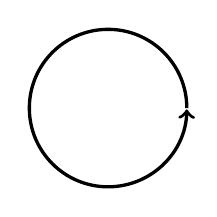
\begin{tikzpicture}
		\draw[->,very thick] (0,0) arc[radius=1cm,start angle=0,delta angle=359];
	\end{tikzpicture}
	\captionof{figure}{\textbf{Ring Gesture \cite{War:2020}}}
\end{center}

\begin{itemize}
	\item Trace a clockwise circle using the wand.
	
	\item Aim again to take around a second to perform the gesture.
	
\end{itemize}

	The steps involved in waving the slope gesture are mentioned below \cite{War:2020}:

\begin{center}
	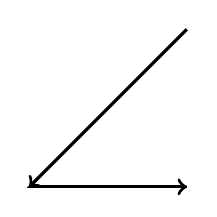
\begin{tikzpicture}
		% define point
		\coordinate (A)  at (2, 2);
		\coordinate (O)  at (0, 0);
		\coordinate (B)  at (2, 0);
		% angle  
		\draw[thick] (A) -- (O) -- (B);
		%\draw pic[draw=black,angle radius=20,angle eccentricity=1.4]
		%{angle = B--O--A};
		%\pic [draw,"$\alpha_1$",angle radius=20,->,angle eccentricity=1.4]
		%  {angle = B--O--A};
		\draw [->, very thick] (2,2) -- (0,0)  node [midway, above] {\scriptsize };
		\draw [->, very thick] (0,0) -- (2,0)  node [midway, above] {\scriptsize };
	\end{tikzpicture}
	\captionof{figure}{\textbf{Slope Gesture \cite{War:2020}}}
\end{center}

\begin{itemize}
	\item The device is first moved down and to the left.
	\item Then the device is moved to the right.
	\item Finally you should get a corner of the triangle as shown in the figure.
\end{itemize}

	The process is repeated until around 15 readings are captured by the wand for Data Preparation and Transformation. 

	In order to consider the unknown readings, we will be carrying out another set of procedures to feed with unknown data. This would help the wand recognize any unknown gesture and give the output that it is false. \cite{War:2020}

	All readings are recorded in a unique text file for each gesture. The files \FILE{.txt} \cite{DataPrep:21} contain raw accelerometer data that would later be transformed into machine learning language that should be interpreted by the compiler. \cite{War:2020}

	Since no existing databases exist for the model, a new database will be created.The database is a .txt file which contains raw data from the accelerometer readings recognized by the board Arduino Nano 33 BLE Sense. Since the way a person records the gesture varies from one to another, the gestures of three people are recorded as we are a group of three members. In order to the database to have a vast amount of data, each person will record at least 50 trials for each gesture. In order for the database to be more accurate data from both hands of the three users were used. This would improve the efficiency and effectiveness of the database making it more concrete. It is also possible to add further data to our model, improving it over time. The size of the database thus created will be petite, less than 2 MB. Obtaining sufficient data is one of the major concerns in a machine learning project and the amount of data involved in our data set is very small. The data thus created will be further used in the next step “Data Preparation and Transformation” where this raw data is further processed and the outliers are identified and removed if necessary.

\section{Data Quantity} 
\subsubsection{Edge Computing}
	The placement of computer and storage resources at the point where data produced is known as edge computing. This computes and stores  the data source at the network edge, which is optimal. In other words, instead of sending raw data to a main data centre for processing and analysis, this work is done right where the data is generated.
	Edge computing is used to handle discrete tasks like determining if someone answered "yes" and responding appropriately. Instead of comparing the data with that on the web, the audio analysis is done on the edge. This drastically decreases expenses and complexity while also reducing the risk of data breaches.\cite{Big:2021}

	Edge computing has gained traction as a viable solution to a variety of issues related to transporting the massive amounts of data that today's businesses generate and consume. It's not just a matter of quantity, it's also a matter of time; applications increasingly rely on processing and responses that are time-sensitive.The analysis and analysis of data produced by connected devices is made possible by edge computing, a crucial element of the Internet of Things (IoT).\cite{Haz:2021} claims that edge computing enables data collecting, processing, and analysis at the network’s edge, facilitating in-the-moment decision-making and minimizing the need to send data to a central point for processing. Edge computing reduces processing times for data, allowing businesses to react swiftly to shifting operational circumstances.

\section{Data Quality}
	Creating a magic wand with board Arduino Nano 33 BLE Sense involves integrating various sensors components and programming logic to ensure data quality for a successful project you need to consider the reliability and accuracy of the data collected from sensors here are some key considerations\cite{Daity:21}.
\subsubsection{Sensor Calibration}
	Sensor calibration calibrate sensors such as accelerometers gyroscopes or magnetometers to ensure accurate readings understand the sensor s specifications and calibrate them accordingly to reduce errors in measurements
\subsubsection{Sensor Fusion}
	Sensor fusion use sensor fusion techniques to combine data from multiple sensors this can improve the accuracy and reliability of the data implement sensor fusion algorithms to obtain a more comprehensive understanding of the wand s orientation and movement
\subsubsection{Wireless Communication Reliability}
	Wireless communication reliability if your magic wand involves wireless communication ensure the bluetooth low energy ble connection is stable and reliable implement error checking mechanisms to handle potential data transmission issues \cite{Gomez:2012}
\subsubsection{Code Optimization}
	Write efficient and optimized code to minimize delays and improve the real-time response of the magic wand.
	Optimize algorithms to reduce processing time and enhance overall system performance.




\section{Data Relevance}
\subsubsection{Real-Time Machine Learning}
	Real Time can be considered as a way of training the model by making it run through live data constantly in order to improve the model. This contradicts the traditional way of machine learning when machine learning engineers were dependent already existent data inputs for creating the model. A method by which we can implement real time learning in to a machine learning model is by continuously feeding it with a data stream and improving the model over time. This is achieved by using an event driven architecture. Event driven architecture is a modern design and development approach that centers about the events occurring in the model. Event-driven architectures create, detect, consume, and react to events.\cite{Haz:2021}. By using a scalable event driven architecture, large number of events in real time can be responded, to which are suitable for loosely coupled softwares(For eg: web services). They also work well with unpredictable and non linear events by making it versatile. \cite{Haz:2021}



\section{Outliers}
	Outliers refer to exceptional or irregular data points that deviate significantly from the expected sensor readings or user interactions. These anomalies can arise from various sources such as sudden movements, extreme sensor values, interference, or unexpected user inputs.outliers in sensor data might occur if the accelerometer or gyroscope registers an unusually rapid or erratic movement that does not align with typical usage patterns. Similarly, outliers in user interaction may manifest as unintended button presses or variations in touch sensor sensitivity.

	Detecting and handling outliers is crucial for ensuring the accuracy and reliability of the magic wand's functionality. Strategies may involve implementing filtering algorithms, calibration techniques, and debouncing mechanisms to mitigate the impact of outliers on sensor readings and user inputs.\cite{Munoz:2019}
\section{Anomalies}
	Creating a magic wand with Arduino Nano 33 BLE involves considering potential anomalies or unexpected behaviors that might arise during the development and usage of the wand. The major challenge while preparing data can be the presence of outliers or anomalies where there are unexpected values. This can be overcome by feeding our model with more data so that the model is efficient.\cite{War:2020}
\begin{itemize}
\subsubsection{Sensor Anomalies}

	\item Accelerometer/Gyroscope Drift
	- Sensors like accelerometers and gyroscopes may experience drift over time, leading to inaccuracies in orientation tracking. Calibration techniques can help mitigate this issue.\cite{Chow:2021}
	\item {Magnetic Interference}
	- Magnetometers can be affected by nearby magnetic fields, leading to anomalies in readings. Shielding or compensation algorithms may be required.
\subsubsection{Power Anomalies}
	\item Unexpected Power Drain
	- Identify and address any unexpected power consumption patterns. Implement power-efficient code and periodically monitor power usage to detect anomalies.
	\item Battery Voltage Fluctuations
	- Voltage fluctuations in the power supply can affect the stability of the Arduino Nano 33 BLE. Implement voltage regulation and monitoring to handle such anomalies. 
\subsubsection{Firmware and Software Anomalies}
	\item Memory Issues
	- Anomalies may occur due to memory limitations on the Arduino Nano 33 BLE. Monitor and optimize memory usage to avoid crashes or unexpected behavior.
	\item Firmware Bugs
	-  Identify and address potential bugs in your firmware. Regular testing, debugging, and code reviews can help mitigate software anomalies.
\end{itemize}
